\section{How ViT Works?}

\begin{frame}{Processing Text}
    \begin{itemize}
        \item \textbf{Token Embeddings}: The input text is broken down into individual tokens (e.g., words, sub-words). Each token is analogous to a patch in an image.
	    \item \textbf{Word Embeddings}: Each token is converted into a fixed-length vector representation (embedding) using a technique like Word2Vec, GloVe, or learned embeddings within the transformer model itself.
	    \item \textbf{Self-Attention on Tokens}: The transformer's self-attention mechanism is applied to these word embeddings. This allows the model to capture relationships between different words in the sentence, understanding context and dependencies.
    \end{itemize}
\end{frame}

\begin{frame}{Processing Images}
    \begin{itemize}
        \item \textbf{Patch Embeddings}: ViT splits an image into fixed-size patches (e.g., 16x16 pixels). Each patch is treated like a token in NLP, much like words in a sentence.
	    \item \textbf{Linear Embedding}: Each patch is flattened into a 1D vector and then linearly projected to a fixed-length embedding.
	    \item \textbf{Self-Attention on Patches}: The Transformer’s self-attention mechanism is then applied to these patch embeddings, allowing the model to learn relationships between patches.
    \end{itemize}
\end{frame}

\begin{frame}{ViT Overview}
    \begin{figure}
        \centering
        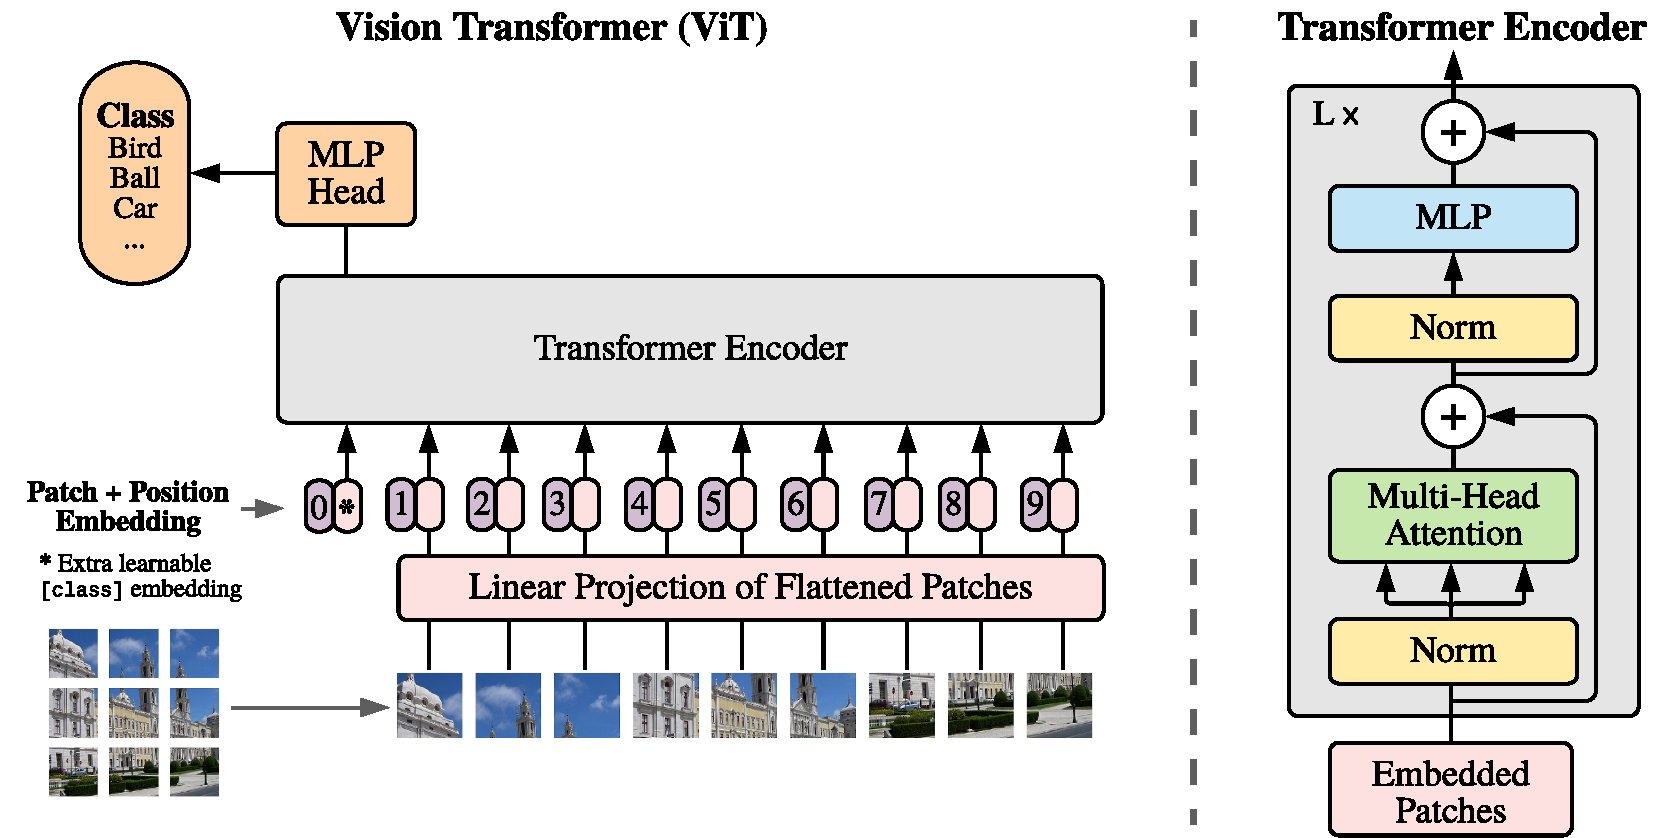
\includegraphics[width=0.95\linewidth]{pic/model_scheme}
        % \caption{We split an image into fixed-size patches, linearly embed each of them, add position embeddings, and feed the resulting sequence of vectors to a standard Transformer encoder. In order to perform classification, we use the standard approach of adding an extra learnable “classification token” to the sequence.}
        \label{fig:vit-figure}
    \end{figure}
\end{frame}

\begin{frame}{Positional Encoding}
    \begin{itemize}
        \item Positional Encoding: Since Transformers process all patches simultaneously (losing the inherent spatial structure of the image), positional encodings are added to the patch embeddings to maintain the relative position of each patch.
	    \item Global Awareness with Position Information: These encodings allow the Transformer to understand not just the content of the patches, but where each patch is located within the image.
    \end{itemize}
\end{frame}

\begin{frame}{Inspecting Vision Transformer}
    \begin{columns}
        \begin{column}{0.5\textwidth}
            \begin{itemize}
                \item Self-attention allows ViT to integrate information across the entire image even in the lowest layers.
            \end{itemize}
        \end{column}
        \begin{column}{0.5\textwidth}
            \begin{figure}
                \centering
                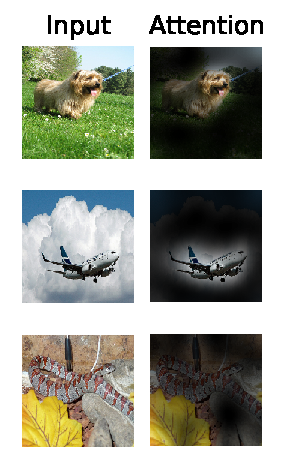
\includegraphics[height=0.75\textwidth]{pic/20201002_selected_attention_examples}
                \caption{Representative examples of attention from the output token to the input space.}
                \label{fig:inspecting-vit}
            \end{figure}
        \end{column}
    \end{columns}
\end{frame}

\begin{frame}{Inductive Bias}
    \begin{itemize}
        \item In CNNs, locality, two-dimensional neighborhood structure, and translation equivariance are baked into each layer throughout the whole model.
        \item In ViT, only MLP layers are local and translationally equivariant, while the self-attention layers are global.
        \item The two-dimensional neighborhood structure is used very sparingly
    \end{itemize}
\end{frame}